\chapter{Data and Processing}

We first assess the preprocessing steps generally used for spike time data, which consists of binning and smoothing spike times to obtain firing rates for each recorded neuron. In sum, we wanted to go from the PSTH figures (or raster plots) to the firing rates. We can see in figure \ref{fig:padding} that applying a gaussian kernel induces correlations between neighboring time points, in such a way that time points with high spike counts induce medium spike counts in neighbour time points. Without smoothing, the activity in single trials is very sparse (i.e. has few nonzero values), and since the precise spike time of a given neuron may not be so representative of its internal state, this transformation into firing rate may aid the classifier in capturing the information present in the neurons.
    
    We can also see, specially when averaging trials, how different paddings result in different estimated firing rates at the borders of the window: padding the activity with zeros biases down the average firing rate. In our posterior analysis, except when explicitly stated, smoothing was done with symmetric padding.
    
    \begin{figure}
        \centering
        \begin{tabular}{cc}
        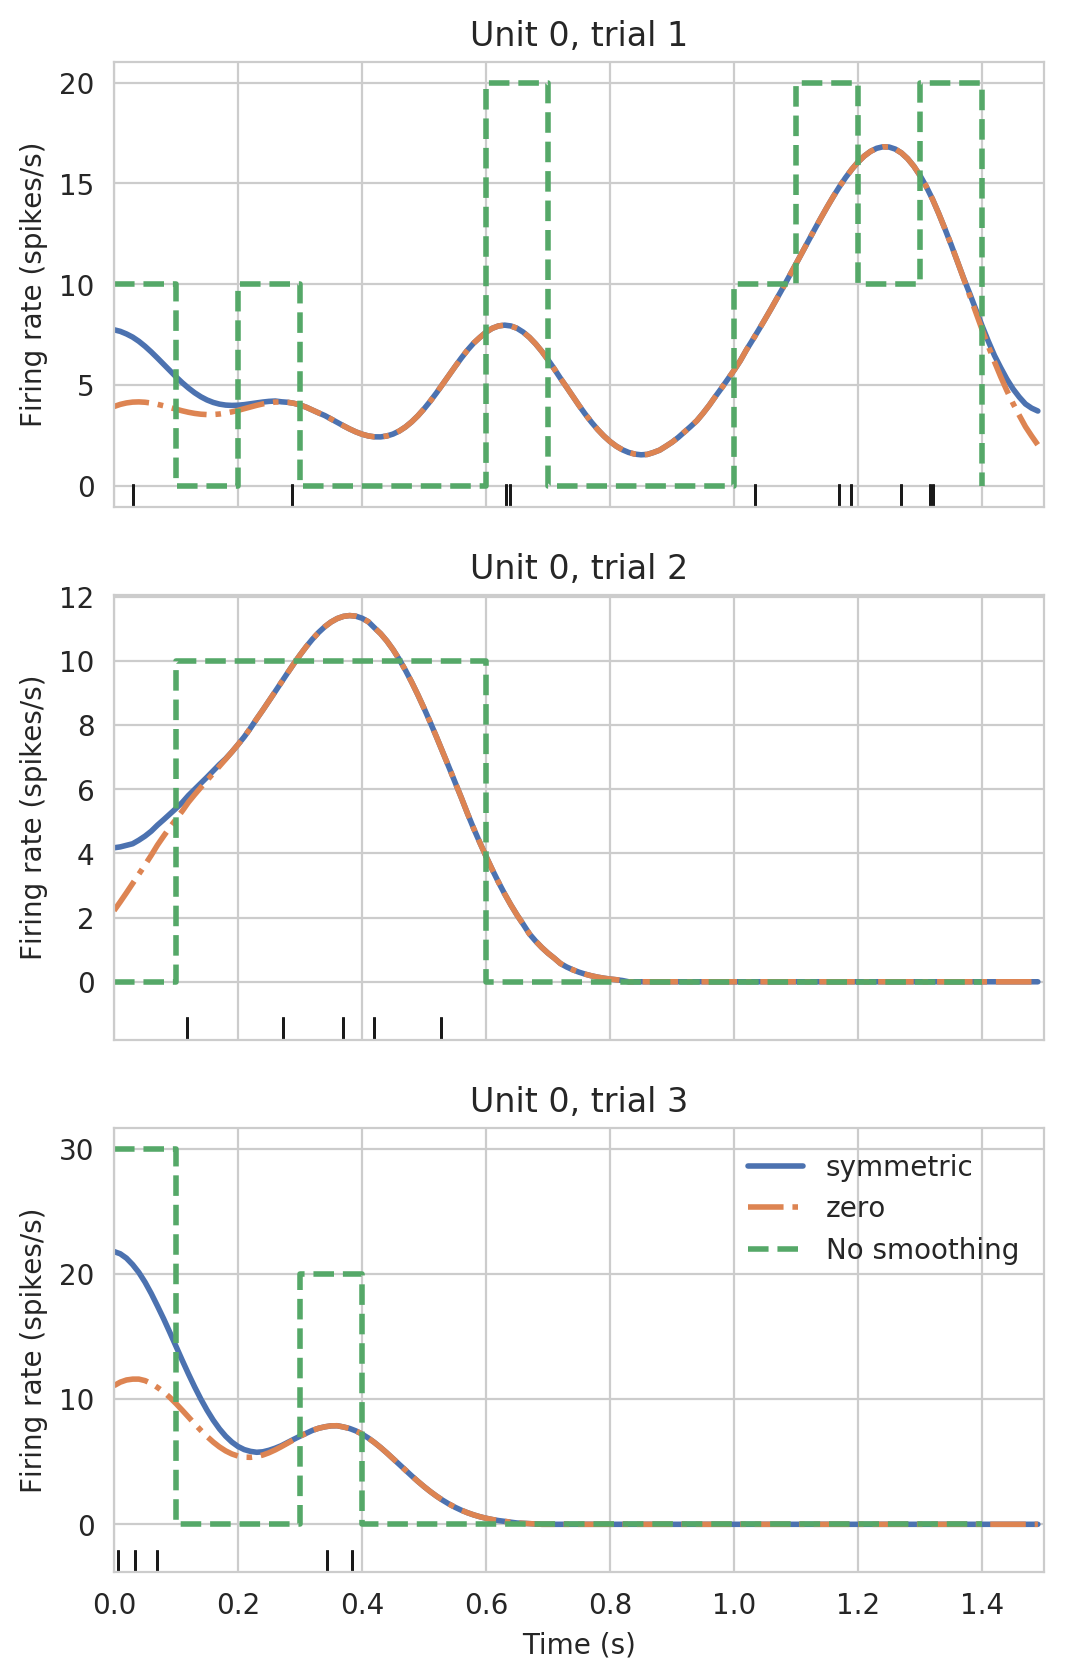
\includegraphics[width=7cm]{figures/one_with_step.png}
        & 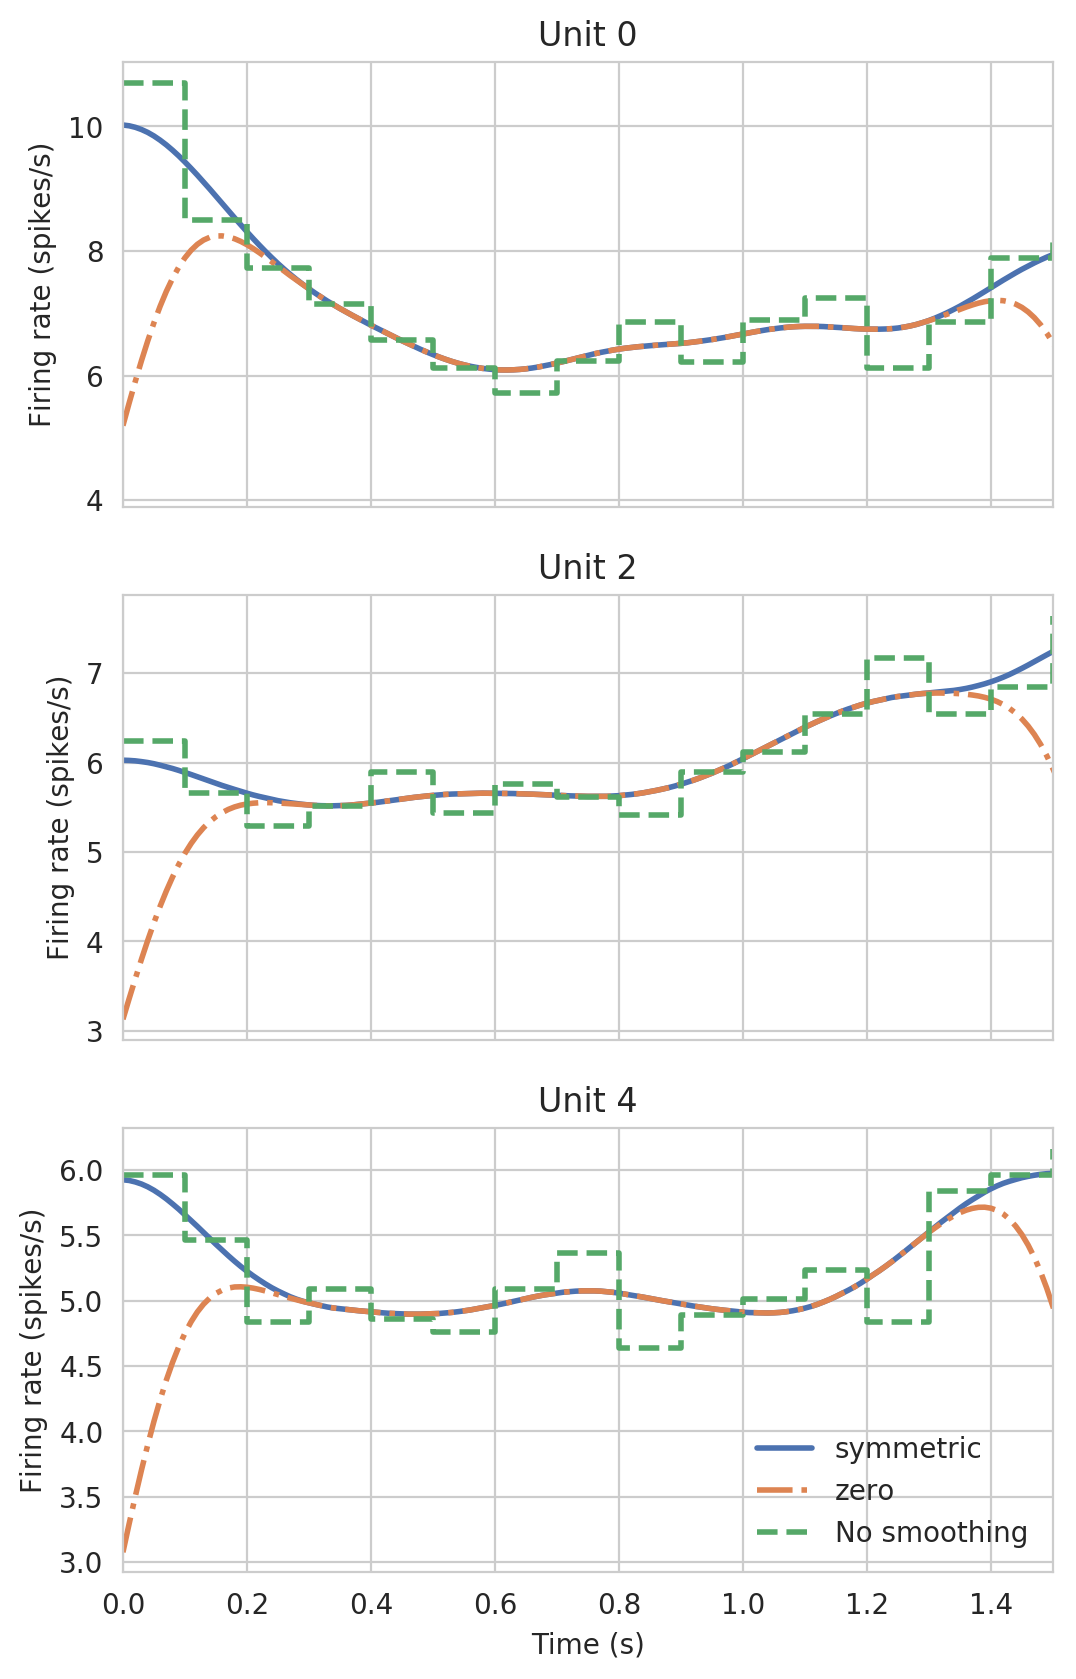
\includegraphics[width=7cm]{figures/mean_with_step.png}
        \end{tabular}
        \caption[Effect of smoothing and padding choices on the estimated firing rate.]{Effect of smoothing the spike counts with a 100ms kernel and padding choices on the estimated firing rate. Left: Single trial firing rates, Right: Mean firing rates. In the left, exact spike times appear as black ticks in the x axis.}
        \label{fig:padding}
    \end{figure} 
    
    \begin{figure}
        \centering
        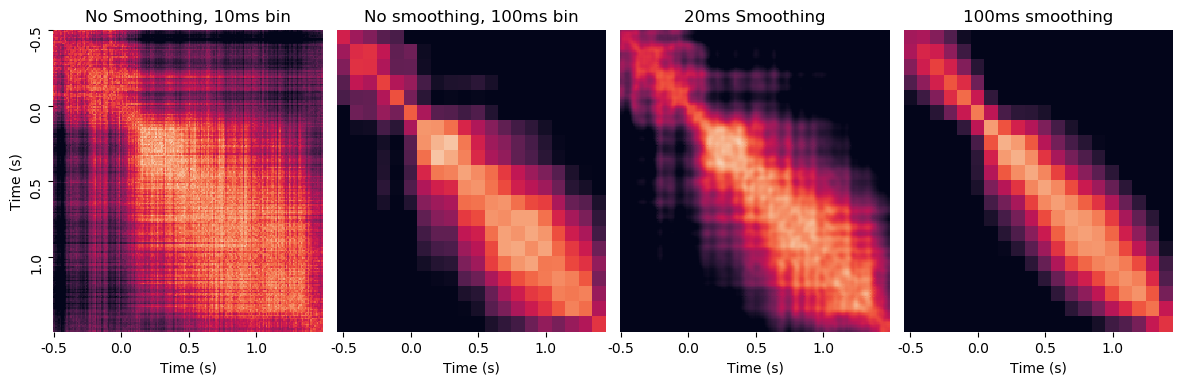
\includegraphics[width=\textwidth]{figures/similarity_comparison.png}
        \caption[Binning and smoothing assessed via similarity matrix]{Binning and smoothing assessed via similarity matrix. Spike count activity at left is binned in small and big time bins, and at the right is smoothed with a narrow and a wide gaussians.}
        \label{fig:mahalanobis_smoothing} 
    \end{figure} %No smoothing, bin10 bin100, DRRD10 and DRRD9
    
    A simple similarity analysis was used in figure \ref{fig:mahalanobis_smoothing} to measure consistency in the dynamics of neural activity. The analysis compares the activity vector of each single time point with the activity vector of another time point, measuring proximity in a space that considers less strongly dimensions in which variability is bigger. We expect to see stronger diagonals when the activity is very similar among trials, indicating that activity vectors coming from the same time point are usually near each other.
    
    In figure \ref{fig:mahalanobis_smoothing}, we can see at the left that bins that are too small can make it hard to see trial consistencies, in the case of no smoothing, because of the sparsity of spike activity. When we bin in 100ms windows, we can see that activity appears more consistent, what can be also achieved by smoothing with small kernels (e.g. 20ms). A larger kernel (100ms) makes the activity yet more consistent. 
    In all cases, it is clear that the baseline is more similar to itself, and different from the rest of the trial. This is expected since the animal is in a different state, generally approaching the nosepoke, as opposed to standing still with its nose inside. 

